\section{Introducción}

%\subsection{Contexto}
La formación musical escolar cumple un rol fundamental en el desarrollo cognitivo y crítico de los estudiantes durante la educación básica y media. Sin embargo, en sistemas educativos en desarrollo como el chileno, la disciplina ha enfrentado una paulatina marginación curricular. Decretos reglamentarios como el N.º 2960 y N.º 628 reducen las horas pedagógicas asignadas a la asignatura a medida que los alumnos avanzan en su trayectoria escolar, obligando a compartir carga horaria con Artes Visuales o relegando la música a un plan electivo \cite{mineduc_decreto2960_2012, mineduc_decreto628_2016}.

%\subsection{Problemática}
Esta restricción horaria genera dos problemas críticos en el aula:
\begin{enumerate}
    \item \textbf{Discontinuidad curricular y heterogeneidad:} La ausencia de linealidad en los planes de estudio provoca que los estudiantes ingresen a niveles superiores con severas lagunas teóricas y niveles de conocimiento muy dispares \cite{chandia_educacion_2025}.
    \item \textbf{Carencia de herramientas pedagógicas adaptadas:} La oferta tecnológica existente (e.g., Yousician, Simply Piano) responde a contextos angloparlantes, aplica itinerarios de aprendizaje rígidos que no respetan la zona de desarrollo proximal del alumno y no provee a los profesores mecanismos de diagnóstico o asignación diferenciada de contenidos \cite{garcia2025, alrowais2025, li2025}.
\end{enumerate}

%\subsection{Pregunta General de Investigación}

Frente al escenario de fragmentación horaria y heterogeneidad presente en la educación musical escolar chilena, surge la siguiente pregunta de investigación:

\textit{¿Puede una tecnología educativa adaptada a la realidad escolar chilena apoyar el proceso de enseñanza y aprendizaje de la teoría musical, favoreciendo una experiencia de aprendizaje más personalizada y efectiva?}

%\subsection{Hipótesis y Propuesta de Solución}

Se plantea como hipótesis que la creación y puesta en marcha de una plataforma web progresiva basada en inteligencia artificial contribuirá positivamente al proceso de enseñanza y aprendizaje de la teoría musical, al ofrecer experiencias adaptadas a las necesidades y ritmo de aprendizaje de cada estudiante.

Para abordar esta hipótesis, el presente trabajo presenta \textit{SheetMusic}, una plataforma web progresiva basada en inteligencia artificial que incorpora técnicas de aprendizaje automático para adaptar de manera dinámica la dificultad y progresión de las actividades de teoría musical a distintos perfiles de estudiantes. La plataforma busca apoyar tanto el aprendizaje autónomo de los estudiantes como el trabajo pedagógico de los docentes mediante herramientas de seguimiento y gestión del progreso académico.

Con el propósito de evaluar la propuesta, se realizó una validación experimental con estudiantes y docentes de la Región de Los Ríos, analizando el impacto de la plataforma sobre el progreso del aprendizaje, la usabilidad del sistema y la percepción de utilidad por parte de sus usuarios.

%\subsection{Casos de Uso del Sistema}

El ecosistema desarrollado considera dos casos de uso principales que representan la interacción de los actores del proceso educativo con la plataforma. La Fig.~\ref{fig:caso_uso_estudiante} muestra las funcionalidades disponibles para los estudiantes, mientras que la Fig.~\ref{fig:caso_uso_profesor} presenta las herramientas orientadas al trabajo pedagógico de los docentes.

\begin{figure}[htbp]
    \centering
    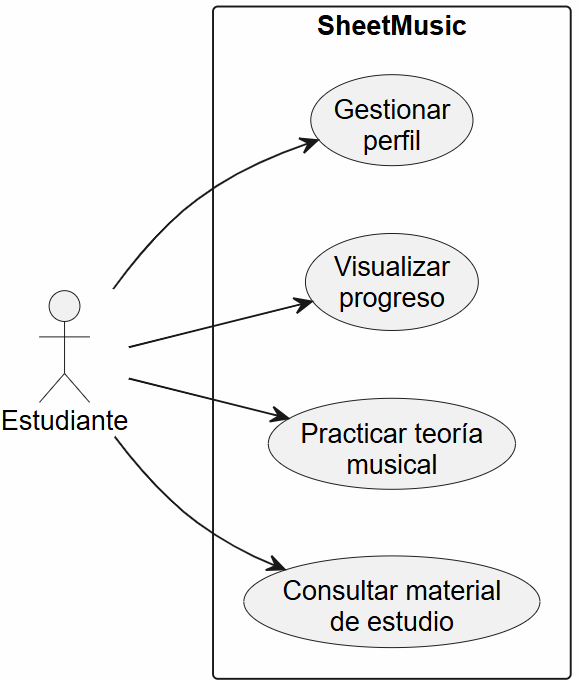
\includegraphics[width=0.28\textwidth]{Imagenes/caso_uso_estudiante.png}
    \caption{Caso de uso principal: interacción del estudiante con el árbol de aprendizaje y resolución de ejercicios adaptativos.}
    \label{fig:caso_uso_estudiante}
\end{figure}

\begin{figure}[htbp]
    \centering
    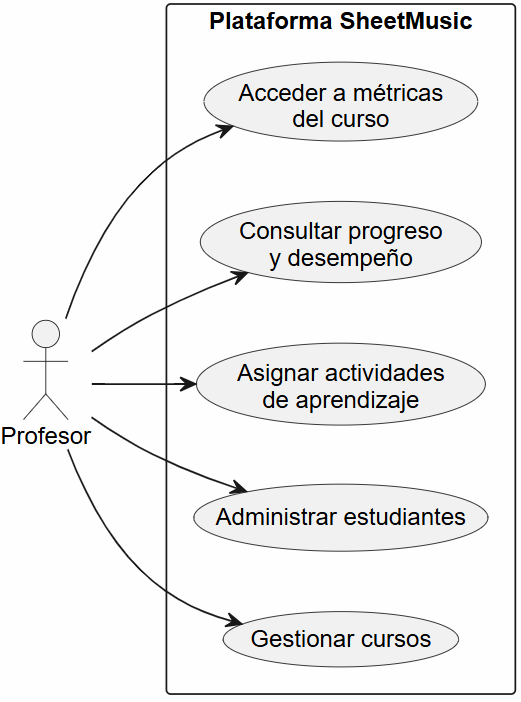
\includegraphics[width=0.28\textwidth]{Imagenes/caso_uso_profesor.png}
    \caption{Caso de uso secundario: módulo de gestión pedagógica y seguimiento docente.}
    \label{fig:caso_uso_profesor}
\end{figure}
En el caso de uso del estudiante (Fig.~\ref{fig:caso_uso_estudiante}), el usuario puede acceder a material de estudio, realizar actividades de aprendizaje relacionadas con la teoría musical, consultar su progreso y administrar su perfil dentro de la plataforma.

Por su parte, el caso de uso del profesor (Fig.~\ref{fig:caso_uso_profesor}) permite gestionar cursos y estudiantes, administrar las actividades de aprendizaje y monitorear el progreso de los estudiantes mediante las herramientas de seguimiento proporcionadas por la plataforma.

Aunque la plataforma contempla funcionalidades para ambos actores, el presente trabajo se centra principalmente en la experiencia de aprendizaje del estudiante y en la evaluación del sistema adaptativo.
%\subsection{Especificación de las Pruebas de Validación}
Para validar la hipótesis planteada, se diseñó un protocolo experimental de 28 días de duración que abarcó dos grupos de usuarios reales de la Región de Los Ríos, Chile:
\begin{itemize}
    \item \textbf{Muestra estudiantil:} 28 estudiantes en total (5 del Conservatorio de Música de la Universidad Austral de Chile y 23 de enseñanza media del Liceo de la comuna de Corral).
    \item \textbf{Muestra docente:} 1 profesor de música en ejercicio para la evaluación del panel pedagógico.
    \item \textbf{Naturaleza de las pruebas:} Se evaluó cuantitativamente la evolución del rendimiento (\textit{proficiency}) guiada por el motor DRL, la usabilidad estudiantil mediante la System Usability Scale (SUS) y la aceptación tecnológica docente a través del Technology Acceptance Model (TAM).
\end{itemize}